\chapter{LDAPとPostfixの連携}

PostfixとLDAPを連携させるときは、Postfixテーブルの参照に対して、LDAPのスキーマを指定します。このとき、ディレクティブに指定するファイルは、1行1レコードのテーブルファイルではなく、探査構文とよばれる、LDAPへのクエリを書いたファイルとなります。

その探査構文の記法について、本章で説明します。

\section{Postfixテーブル}

PostfixテーブルをLDAPに置くとき、基本的な戦略は、テーブルと対応づけた子ノードとして、レコードに相当するノードを置きます。また、この探索においては、再帰が生じないように、レコードに相当するものは、全て兄弟ノードとします。つまり、Postfixテーブルは、親と複数の子だけからなぶ部分木として、LDAPツリーの中に存在させます。

\subsection{LDAPへの置き換え}
Postfixテーブルは、mail.cf(5)の中で、テーブル名と、参照スキーマ、定義ファイルのパスをイコールで結んで設定します。
参照スキーマのスキーマという用語は、LDAPのオブジェクトタイプ定義ではなく、データにアクセスする手段としてのスキーマとして使われています。ここでは、hash:というのが、ハッシュテーブルを参照する、というスキーマになります。
例として、、エイリアスをハッシュテーブル形式で記述する設定を書いてみましょう。

\begin{verbatim}
alias_maps = hash:/etc/postfix/alias
\end{verbatim}

ここで、aliasというのは、Postfixテーブル形式で書いたテキストファイルの名前です。実際には、postmap(8)コマンドでハッシュした結果の、alias.dbというファイルが参照されます。

\subsection{LDAPスキーマによるアクセス}

LDAPに置いたエイリアス情報を参照する場合、この設定は以下のように書きます。

\begin{verbatim}
alias_maps = ldap:/etc/postfix/ldap_alias
\end{verbatim}

alias\_mapsディレクティブの右辺には、LDAPの探査構文を書いたテキストファイルを指定します。参照スキーマがLDAPのときは、指定されたファイルは、LDAPの探査構文を指定したファイルとなります。探査構文の例を示します。

\begin{verbatim}
search_host = ldap.uranohoshi.example
search_base = ou=aliases,ou=tables,dc=uranohoshidc=example
bind = yes
bind_dn = cn=Manager,dc=uranohoshi,dc=example
bind_pw = password
scope = one
query_filter = (&(mail=%s)(mailEnalbe=OK))
result_attribute = maildrop
result_format = %s
\end{verbatim}

\subsection{探索の戻り値}

\begin{figure}[htbp]
	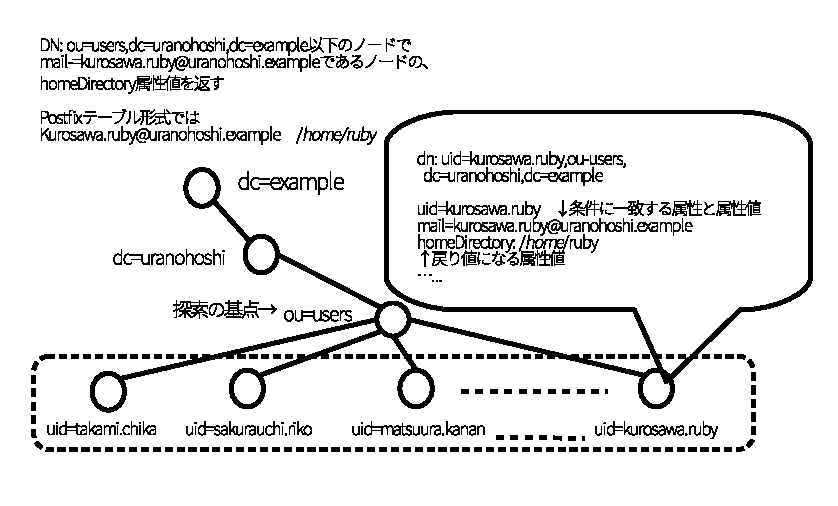
\includegraphics[width=12cm,clip]{draw/search.eps}
	\caption{LDAPの探索}
	\label{fig:`search}
\end{figure}

LDAPでも、Postfixテーブルと同様に、クエリに合致するノードが見つかったら、戻り値として指定した属性の属性値が返されます。通常、クエリにはマクロで探索のキーを与えます。このキーが、Postfixテーブルの左辺に相当します。また、また、返される属性値がPostfixテーブルの右辺に相当します。

キーが探索できない場合は、該当する結果がないと言うことになり、この点もPostfixテーブルによる探索とかわりません。


\subsection{探査構文ファイルのディレクティブ}

探査構文ファイルは、LDAPサーバの情報と、その中で情報を探すのに必要な情報とが書かれています。そのディレクティブの主なものについて説明します。

\paragraph{search\_host}
アクセスするLDAPサーバを、解決可能な名前もしくはIPアドレスで指定します。LDAPスキーマはネットワーク透過であり、LDAPサーバはPostfixと同じホストの上になくてもかまいません。

\paragraph{search\_base}
DITの中で、このノードを起点に探索を行う、場所を指定します。ルートからのDNで記載します。

\paragraph{bind}
何らかのユーザ認証を行った上でDITにアクセスするかのフラグです。yesかnoで記述します。
noの場合は、探査の対象となる部分が、LDAPサーバの設定で、匿名でアクセス可能になっている必要があります。

\paragraph{bind\_dn}
ユーザ認証を行うとき、そのユーザの情報が入っているノードをDNで指定します。この例では、LDAPの管理アカウントを指定しています。

\paragraph{bind\_pw}
ユーザ認証に使うパスワードを記述します。プレーンテキストで記述するので、メールサーバのOSの設定で、探査構文ファイルのアクセス権を適切に設定する必要があります。

\paragraph{scope}
base\_dnを起点に、土の範囲を探すかを指定します。oneを指定した場合は、base\_dnと、その直接の子ノードのみを探索の対象とします。
subを指定した倍は、base\_dnと、それを起点とする部分木全てが探索の対象となります。このディレクティブを省略した時のデフォルト値は、subになります。

\paragraph{query\_filter}
LDAPに問い合わせを行うときのクエリ構文です。詳細は次の章で解説します。

\paragraph{result\_attribute}
戻り値となる属性を指定します。探索に一致するノードがあれば、そのノードの、属性値が全てが返されます。

\paragraph{result\_format}
戻り値のフォーマットを設定します。result\_attributeで指定した属性の値をそのまま使う場合は、省略可能です。例えば、以下のように記述すると、属性値を、DNSでMX探索を行わず、そのままsmtpサービスによる宛先とするホスト名、というように、Transport(5)テーブルの戻り値となります。

\begin{verbatim}
result_format = smtp:[%s]
\end{verbatim}

\section{探査構文のクエリと結果}



LDAPの探索を行うとき、探索の基点となるDNから、キーとなる属性と、その属性値のペアを持つノードがないかを探します。この探索は、基点となるノードと、その子ノード、もしくは、基点から下の部分木となります。

もし、探索のキーとなる、属性と属性値のペアを持つノードがあれば、そのノードが、戻り値とする属性を持っているかをチェックします。その属性があれば、属性値が戻り値となります。
キーと一致する属性と属性値のペアを持つノードがない、もしくは、戻り値として指定した属性がない場合、戻り値はありません。これは、Postfixテーブルで、該当するレコードがない状況に相当します。

\subsection{クエリの記述}

探査構文の中で、query\_filterは、LDAPで該当するノードがあるかどうかを探すための構文となります。この構文は、属性と、属性値のペアをセットを丸括弧で囲って記述します。
たとえば、属性mailEnableの属性値がOKであるノードがあるかを探すときは、以下のように記述します。

\begin{verbatim}
query_filter = (mailEnable=OK)
\end{verbatim}

また、この探索では、AND、OR,NOTが使用可能です。これは、演算子を前におく、前置記法(ポーランド記法)で記述します。属性mailEnableがOKでないノードを条件とする伊ときは、NOT演算子!をつけます。

\begin{verbatim}
query_filter = (!(mailEnable=OK))
\end{verbatim}

\%sという入力キーを著わすマクロを使って、それがmail属性に一致して、mailEnable属性がOKであるノードがあるかを探すには、以下のように書きます。AND演算子として、\&を用います。

\begin{verbatim}
query_filter = (&(mail=%s)(mailEnable=OK))
\end{verbatim}

OR演算子は
\textbar
になります。以下のように記述します。mailEnableの属性値がdisabledか、defferかのどちらかであるノードとヒットします。

\begin{verbatim}
query_filter = (|(mailEnalbe=disabled)(mailEnable=deffer))
\end{verbatim}



\subsection{戻り値の加工}

LDAPの属性値は、そのままPostfixテーブルのフォーマットになっているとかは義理ません。特に、汎用のユーザアカウントデータベースを参照している場合は、Postfixのみで使うフォーマットで属性値を記述するべきではない、ということでもあります。

そのため、result\_formatで、戻り値のフォーマットを設定することができます。result\_attributeでしていた属性の、戻り値となる属性値がメールアドレス形式であるとすれば、@の左のアドレスを著わすマクロ\%uと、右のドメイン部分を著わす\%dが使えます。

れいとして、バーチャルドメイン運用の時、メールアドレスとそのメールアドレスを格納するディレクトリのパスの万ピングテーブルである、virtual\_mailbox\_maxpの探査構文は、以下のようになります。

\begin{verbatim}
# Maildir/運用のときのマッピング
query_filter = (mail=$s)
result_attribute = mail
result_format = /home/%u/Maildir/
\end{verbatim}

特定のドメイン宛のメールを、別のメールサーバに転送する、transport(5)のための探査構文は、以下のように書けるでしょう。
domainと、nexthopという二つの属性は、transport(5)のために定義した属性であるとします。戻り値となる属性値は、\%sであらわされます。

\begin{verbatim}
query_filter = (domain = %d)
result_attribute = nexthop
result_format = smtp:[%s]
\end{verbatim}

\subsection{探査構文で使用できるマクロ}

LDAPの探査構文では、入力値と、その部分を著わすマクロを使用することができます。このマクロは、base\_dn、query\_filter、result\_formatで使用することができます。

\paragraph{\%s}
入力キーをあらわすマクロです。base\_dnとquery\_filterでは、テーブル左辺に相当する探索のキーをあらわします。
result\_formatでは、一致するノードがあって戻り値があるとき、その戻り値として指定された属性値そのものをあらわします。

\paragraph{\%u}
マクロ\%sの内容が、mari@uranohoshi.exampleのようなメールアドレス形式であるとき、@から左側がその値となります。

\paragraph{\%d}
マクロ\%sの内容がメールアドレス形式であるとき、@から右の、ドメイン名もしくはホスト名部分が、その値となります。

\paragraph{\%[1-9]}
マクロ\%sの内容がメールアドレス形式であるとき、@から左のドメイン部分が、ドット区切りの右から順番に、1、2,というように割り当てられます。dia@mail.uranohoshi.exampleというメールアドレスがキーの場合、\%1はexample、\%2はuranohoshi、\%3は、mailとなります。

このマクロは、ひとつのDITに複数ドメインの情報を入れた場合、探索の起点であるbase\_dnを選択する、というような場合に使います。

\begin{verbatim}
base_dn = ou=users,dc=%2,dc=%1
\end{verbatim}

\section{レコードの置き換え}
Postfixテーブルのレコードを、LDAPに置き換えてみましょう。今度は、transport(5)をLDAPに置き換えてみます。

\subsection{transport(5)}

transport(5)は、届いたメールをどのような手段でネクストホップに転送するかを、メールアドレスもしくはドメイン名を左辺に、転送先と転送に使うサービスを右辺に記述します。

main.cf(5)で、transportテーブルは以下のように定義されているとします。

\begin{verbatim}
transport_maps = hash:/etc/postfix/transport
\end{verbatim}

この場合、/etc/postfix/transportをハッシュした、transport.dbというファイルが参照されます。
ハッシュされるものとファイルには、以下のように書いてあるとしましょう。

\begin{verbatim}
otonoki.example  smtp:[mailgw.otonoki.example]
aqours@uranohoshi.example  smtp:[aqours.uranohoshi.example]
uranohoshi.example    smtp:
\end{verbatim}

内容としては、以下のようになります。

\begin{enumerate}
  \item otokonoki.exampleドメイン宛のメールは、ゲートウェイサーバmailgw.otonoki.exampleに転送
  \item aqours@uranohosshi.example宛のメールは、専用サーバaqours.uranohoshi.exampleに転送
  \item それ以外のuranohoshi.exampleドメイン宛のメールは、DNSでMX検索して転送
\end{enumerate}、

転送はいずれも、master.cf(8)で定義されているsmtpサービスを使います。また、transport(8)はファーストマッチなので、上から適合するものが用いられます。

\subsection{Transportテーブル置き換えのスキーマ}
TransportテーブルをLDAPのノードにするために、その左辺と右辺をあらわす属性を定義しましょう。結論から行くと、以下のようなスキーマファイルで著わされます。

以下のスキーマでは、OIDのPENとして、99999を使用しています。これはIANAによって割り当てられた数字ではなく、説明用に使用しているものです。実際に、独自のスキーマを定義素して使用するときは、IANAからPENを取得するようにしてください。

\begin{verbatim}
attributeTypes: ( 1.3.6.1.4.1.99999.1.1
        NAME 'transportSource'
        DESC 'Postfix Transport(5) source'
        EQUALITY caseIgnoreMatch
        SUBSTR caseIgnoreSubstringsMatch
        SYNTAX 1.3.6.1.4.1.1466.115.121.1.15 )


attributeTypes: ( 1.3.6.1.4.1.99999.1.2
        NAME 'transportDestination'
        DESC 'Postfix Transport(5) destination'
        EQUALITY caseIgnoreMatch
        SUBSTR caseIgnoreSubstringsMatch
        SYNTAX 1.3.6.1.4.1.1466.115.121.1.15 )


objectclass (1.3.6.1.4.1.99999.1
        Name 'postfixTransport'
        DESC 'Postfix tranport table object'
        SUP top
        STRUCTURAL
        MAY ( transportSource $ transportDestination ) )
\end{verbatim}

このスキーマファイルは、transportSource、transportDextinationという二つの属性を、オブジェクトタイプpostfixTransportとして、追加します。どちらも、メールアドレスではなく、属性値が文字列であるとして定義しています。

また、オブジェクトタイプpostfixTransportを利用して、transport(5)相当のLDIFを、以下のように定義します。

\begin{verbatim}
dn: tranportSource=otonoki.ecample,ou=transport,
   ou=tables,dc=uranohoshi,dc=example
changeType: add
objectClass: top
objectClass: postfixTransport
transportSource: otonoki.example
transportDestination: smtp:[otonoki.example]

dn: tranportSource=aqours@uranohoshi.example,ou=transport,ou=tables,
   dc=uranohoshi,dc=example
changeType: add
objectClass: top
objectClass: postfixTransport
transportSource: aqours@uranohoshi.example
transportDestination: smtp:[aqours.uranohoshi.example]

dn: tranportSource=uranohoshi.example,ou=transport,ou=tables,
   dc=uranohoshi,dc=example
changeType: add
objectClass: top
objectClass: postfixTransport
transportSource: aqours@uranohoshi.example
transportDestination: smtp:

\end{verbatim}

\subsection{まちがった探査構文定義}

transport(5)のかわりとなる部分木にアクセスするには、どのような探査構文を定義すれば良いでしょうか。
まず、動きそうだけど期待通り動かない場合がある例を示します。

\begin{verbatim}
search_host = ldap.uranohoshi.example
search_base = ou=transport,ou=tables,dc=uranohoshidc=example
bind = yes
bind_dn = cn=Manager,dc=uranohoshi,dc=example
bind_pw = password
scope = one
query_filter = (|(transportSource=%s)(transportSource=%d))
result_attribute = transportDestination
result_format = %s
\end{verbatim}

この探査構文のファイル名が、transport.cfであるとすると、main.cf(5)では、このように定義されます。

\begin{verbatim}
transport_maps = ldap:/etc/postfix/transport.cf
\end{verbatim}

一見すると、これでトランスポートテーブルになりそうです。ですが、これは期待通りに動きません。それは、aqours@uranohoshi.exampleに適用される転送ルールと、uranohoshi.exampleに適用されるルールのどちらが先に判定されるか、確定できないためです。

そのため、この探査構文の定義では、aqours@uranohoshi.example宛てのメールが、専用サーバaqours.uranohoshi.netに転送される場合と、権威DNSに登録されている、uranohoshi.exampleのMXのどちらに転送されるかが確定しません。

つまり、この例では先にメールアドレスのマッチングが先に試みられる必要があります。

\subsection{正しい探査構文}

では、正しい順番で判定する探査構文とはどのようなものでしょうか・まず、探査構文を、transportSourceにメールアドレスがきているとして、探索を行うものと、ドメイン名がきているときに探索を行うものとに分けます。

まず、メールアドレスについて探査する探査構文ファイルを、transport\_mail.cfとします。

\begin{verbatim}
search_host = ldap.uranohoshi.example
search_base = ou=transport,ou=tables,dc=uranohoshidc=example
bind = yes
bind_dn = cn=Manager,dc=uranohoshi,dc=example
bind_pw = password
scope = one
query_filter = (transportSource=%s)
result_attribute = transportDestination
result_format = %s
\end{verbatim}

同様に、ドメインについて探索する探査構文ファイルを、transport\_domain.cfとします。

\begin{verbatim}
search_host = ldap.uranohoshi.example
search_base = ou=transport,ou=tables,dc=uranohoshidc=example
bind = yes
bind_dn = cn=Manager,dc=uranohoshi,dc=example
bind_pw = password
scope = one
query_filter = (transportSource=%d)
result_attribute = transportDestination
result_format = %s
\end{verbatim}

つぎに、main.cf(5)で、transport\_mapsディレクティブを設定します。ここで、main.cfのディレクティブは、ファーストマッチであることを利用します。先にメールアドレスによる探査構文を参照させ、それで見つからない場合に、ドメインの探査構文を適用させます。

\begin{verbatim}
transport_maps = ldap:/etc/postfix/transport_mail.cf
                 ldap:/etc/postfix/transport_domain.cf
\end{verbatim}

\subsection{すべてのPostfixテーブルをLDAPに乗せるべきか}

transport(5)をLDAPに乗せるのは、少しばかり問題があることがわかりました。今回は、メールアドレスによるルールは、ドメイン名によるルールよりも優先度が高い、ということで対処できました。
ですが、この優先順が一意に定まらない場合など、無理にLDAPに乗せないほうが運用しやすい場合もあります。

その場合は、テキストファイルをベースとする運用をするほうが簡単でしょう。